% This template  originally from Paul Goldsmith-Pinkham: https://github.com/paulgp

\documentclass[11pt]{article}
\usepackage[top=0.8in, bottom=0.78in, left=0.87in, right=0.87in]{geometry}
\usepackage{setspace}
\usepackage[T1]{fontenc}
\usepackage{times}
\usepackage{booktabs}
\usepackage{rotating}
\usepackage{graphicx}
\usepackage[section]{placeins} %Placeins.sty keeps floats `in their place', preventing them from floating past a "\FloatBarrier" command into another section.  To use it, declare "\usepackage{placeins}" and insert "\FloatBarrier" at places that floats should not move past, perhaps at every "\section".  
\usepackage[large, bf]{caption}
\usepackage[FIGTOPCAP]{subfigure}
\usepackage{pdfpages}
\usepackage{palatino}
\usepackage{pdflscape}
\usepackage{textcomp}
\usepackage{longtable}
\usepackage{nicefrac}
\usepackage{adjustbox}	% to adjust the size of objects to fit into a page
\usepackage[hyphens]{url}

\usepackage{natbib}
\bibpunct{(}{)}{;}{a}{,}{,}

\def\citeapos#1{\citeauthor{#1}'s (\citeyear{#1})}

%zero spacing between references
%\usepackage{bibspacing}
%\setlength{\bibspacing}{\baselineskip}

%%-----------------------------------------------------------------
%%Header
%\usepackage{fancyhdr}
%\fancyhf{}
%\fancyhead[C]{\textit{Preliminary and Incomplete}}
%\fancyfoot[C]{\thepage}
%\renewcommand\headrulewidth{0pt}
%\pagestyle{fancy}
%%-----------------------------------------------------------------

%\onehalfspacing
\doublespacing

\usepackage{amsmath, amsfonts, amssymb, amsthm}

%\usepackage{mathpazo} %Use Palotino fonts
\parskip 0ex  %Vertical distance between paragraphs, in "ex"s
\parindent 20pt

%\usepackage{harvard}
%\bibliographystyle{apsr}
%\bibliographystyle{dcu}

\usepackage[pdftex]{hyperref}
\hypersetup{colorlinks, citecolor=blue, filecolor=blue, linkcolor=blue, urlcolor=blue}

\newtheorem{theorem}{Theorem}
\newtheorem{lemma}{Lemma}
\newtheorem{proposition}{Proposition}
\newtheorem{corollary}{Corollary}
\newtheorem{prediction}{Prediction}
\newtheorem{case}{Special Case}

\newenvironment{proofAlt}[1][Proof]{\begin{trivlist}
\item[\hskip \labelsep {\bfseries #1}]}{\end{trivlist}}
\newenvironment{definition}[1][Definition]{\begin{trivlist}
\item[\hskip \labelsep {\bfseries #1}]}{\end{trivlist}}
\newenvironment{example}[1][Example]{\begin{trivlist}
\item[\hskip \labelsep {\bfseries #1}]}{\end{trivlist}}

\newenvironment{remark}[1][Remark]{\begin{trivlist}
\item[\hskip \labelsep {\bfseries #1}]}{\end{trivlist}}
\def\urltilda{\kern -.15em\lower .7ex\hbox{\~{}}\kern .04em}

\renewcommand{\thesubfigure}{(\Alph{subfigure})}

%%%%%%%%%%%%%%%%%%%%%%%%%%%%%%%%%%
% SPACING
%%%%%%%%%%%%%%%%%%%%%%%%%%%%%%%%%%

\usepackage{titlesec}

\titlespacing*{\section}{0pt}{1.5ex plus 1ex minus .2ex}{0.8ex plus .2ex}
\titlespacing*{\subsection}{0pt}{1.2ex plus 1ex minus .2ex}{0.8ex plus .2ex}
% Decimal align 
\usepackage{dcolumn}
\newcolumntype{d}[0]{D{.}{.}{5}}

\usepackage{graphicx}
\graphicspath{{../../output/}}
\usepackage[]{epstopdf}
% This adds the output directory to the inputs function (code outputs are latex inputs!) so you don't have to use a relative path each time
\makeatletter
\providecommand*{\input@path}{}
\g@addto@macro\input@path{{../../output/}}% append
\makeatother


\usepackage[space]{grffile}

 
\title{\textbf{\LARGE{PAPER TITLE}}\thanks{First version: DATE. This version: \today.  ACKNOWLEDGEMENTS HERE}}

\author{
	AUTHOR 1\thanks{UNIVERSITY 1. Email: \href{mailto:author@address.com}{author@address.com}} \and
	AUTHOR 2\thanks{UNIVERSITY 2. Email: \href{mailto:author@address.com}{author@address.com}} \and 
	AUTHOR 3\thanks{UNIVERSITY 3. Email: \href{mailto:author@address.com}{author@address.com}} \and 
	AUTHOR 4\thanks{INSTITUTION 1. Email: \href{mailto:author@address.com}{author@address.com}} 
	}
			
\date{\today}

\begin{document}

\maketitle
\thispagestyle{empty} 
\setcounter{page}{0}

\begin{abstract}
ABSTRACT HERE

\end{abstract}


	  
%%%%%%%%%%%%%%%%%%%%%%%%%%%%%%%%%
% Text
%%%%%%%%%%%%%%%%%%%%%%%%%%%%%%%%%
	
\clearpage

\section*{Overall Contribution}
\textit{This was shared by Ravi Kudesia from an unknown `reviewer 3'. I've paraphrased it a bit:}\\ 
When I look at your paper, I ask myself the following two questions:
\begin{enumerate}
\item How does the manuscript change, challenge, or fundamentally advance our knowledge of the concepts, relationships, models, or theories embedded in the literature
on X?
\item How does the manuscript cause us to think about X in a way that would not normally be anticipated from extrapolations of existing work, thereby advancing future work in an important and useful way?
\end{enumerate}
X is the literature to which you want to contribute. 

In response to question 1, I often find it useful to create a 3x4 matrix. On one side I list
(1) change, (2) challenge, and (3) fundamentally alter. On the other side I list (1)
concepts, (2) relationships, (3) models, and (4) theories. 

Theoretically, you have simply not laid out what main insight your paper generates. You
need to say much more about why your paper is a useful and substantial contribution.
One way to rethink the structure and contribution of your paper is to answer the 10
questions listed in Table 3 on page 757 in Patriotta, G. 2017. Crafting Papers for
Publication: Novelty and Convention in Academic Writing. Journal of Management
Studies. The 10 questions are:

\begin{enumerate}
\item This is what I am focusing on
\item This is why it is relevant
\item This is what is known/not known (and why it needs attention)
\item This is my burning question
\item This is how I aim to address the question (theoretically/empirically)
\item This is what I did
\item This is what I found
\item This is what it means
\item This is what I add
\item This is why you should care
\end{enumerate}

Create a document and use the 10 questions as headlines, and then write your answer
below each question. You already have the answer to many of the questions. The total
document should not be longer than 2 or 3 pages. This approach will help you to
develop your argument.


\section{Introduction}
\textit{Tips on introductions taken from Keith Head's introduction formula (in turn informed by John Ries and Jim Brander):}
\begin{enumerate}
\item \textbf{Hook}: Attract the reader's interest by telling them that this paper relates to something interesting. What makes a topic interesting? Some combination of the following attributes makes Y something worth looking at.
\begin{itemize}
\item Y matters: When Y rises or falls, people are hurt or helped.
\item Y is puzzling: it defies easy explanation.
\item Y is controversial: some argue one thing while other say another.
\item Y is big (like the service sector) or common (like traffic jams).
\end{itemize}
Things to avoid: 
\begin{itemize}
\item The bait and switch : promising an interesting topic but delivering something else, in particular, something boring.
\item ``all my friends are doing it'' : presenting no other motivation for a topic than that other people have written papers on it.
\end{itemize}

\item \textbf{Question}: Tell the reader what this paper actually does. Think of this as the point in a trial where having detailed the crime, you now identify a perpetrator and promise to provide a persuasive case. The reader should have an idea of a clean research question that will have a more or less satisfactory answer by the end of the paper. Examples follow below. The question may take two paragraphs. At the end of the first (2nd paragraph of the paper) or possibly beginning of the second (3rd paragraph overall) you should have the ``This paper addresses the question'' sentence.

\item \textbf{Antecedents}: Identify the prior work that is critical for understanding the contribution this paper will make. The key mistake to avoid here are discussing papers that are not essential parts of the intellectual narrative leading up to your own paper. Give credit where due but establish, in a non-insulting way, that the prior work is incomplete or otherwise deficient in some important way.

\item \textbf{Value-Added}: Describe approximately 3 contributions this paper will make relative to the antecedents. This paragraph might be the most important one for convincing referees not to reject your paper. A big difference between it and the earlier ``question'' paragraph is that the contributions should make sense only in light of prior work whereas the basic research question of the paper should be understandable simply in terms of knowing the topic (from the hook paragraph). John suggests that ``Antecedents'' and ``Value-added'' may be intertwined. They may also take up to 3 paragraphs.

\item \textbf{Road-map}: Outline the organization of the paper. Avoid writing an outline so generic that it could apply to any paper (``the next section is the middle of the paper and then we have the end''). Instead customize the road map to the project and possibly mention pivotal ``landmarks'' (problems, solutions, results…) that will be seen along the way. But keep this short because many readers will now be eager to get to the heart of the paper.
\end{enumerate}

\section{The middle bits}
\textit{From a blog post by Marc Bellemare and edited down a bit:}\\
Let’s look into the outline of the typical paper. When I write a new paper, the first thing I do in LaTex is to create the following sections:
\begin{itemize}
\item Introduction
\item Theoretical Framework
\item Empirical Framework
\item Data and Descriptive Statistics
\item Results and Discussion
\item Conclusion
\end{itemize}
The ``middle bits'' are everything that is not the introduction or the conclusion, so here is a formula for those. Now, I am not saying ``here is the right formula for those''; this is something that has worked for me by reducing the amount of uncertainty I face when writing the typical paper. Let's flesh out each section.

\subsection{Theoretical Framework}
\begin{itemize}
\item \textbf{Primitives}: What are the preferences and/or technology like?
\item \textbf{Variables}: What are the choice (i.e., theoretically endogenous) variables? What are the parameters (i.e., theoretically exogenous variables)?
\item \textbf{Assumptions}: What assumptions are you making about preferences and/or technology? What assumptions are you making about the choice variables? What assumptions are you making about the parameters?
\item \textbf{Maximisation Problem}: What are the agents you are studying maximizing? What is the Lagrangian?
\item \textbf{First-Order Conditions}: Self-explanatory. In some cases where it is not obvious that you are solving for a maximum or a minimum, you’ll want to show the second-order conditions as well.
\item \textbf{Testable Prediction}: State your main testable prediction. Generally, this should map one-to-one with the empirical framework.
\item \textbf{Proof}: Prove your main testable prediction. Here, go for simplicity rather than elegance–why go for a proof by construction when a proof by contradiction will do just fine?
\item \textbf{Other Results and Proofs}: There might be some side results you can both demonstrate in theory and test empirically. Generally, I think one paper should do one big thing–but there are exceptions.
\end{itemize}

\subsection{Empirical Framework}
\begin{itemize}
\item \textbf{Estimation Strategy}: What equations will you estimate? How will you estimate them? How will you treat the standard errors? What is the hypothesis test of interest for your main testable prediction? This is why there should generally be a one-to-one mapping from the main testable prediction to the empirical framework. If your outcome variable or variable of interest needs to be constructed or estimated, this is where you'd discuss it.

\item \textbf{Identification Strategy}: What would the ideal data set look like to study your question? How close are you to that ideal, and what prevents you from getting closer? Then, discuss in turn how your identification strategy deals or not with (i) unobserved heterogeneity, (ii) reverse causality or simultaneity, and (iii) measurement error. Also think about what a violation of the stable unit treatment value assumption looks like here (does one observation getting treated somehow affect the outcome of another observation?), and whether you can somehow test for it.
\end{itemize}

\subsection{Data and Descriptive Statistics}
\begin{itemize}
\item \textbf{Data}: When was it collected? Where? Why? By whom? How was the sample selected? Who was interviewed, or how were the data collected? What is the sample size? How does it compare to the population of interest? Do you lose any observations? Why? Did you have to impute any values and, if so, how did you do it? Are any variables proxies for the real thing? What does each variable measure, exactly, or how was it constructed?

\item \textbf{Descriptive Statistics}: This is simple enough. If you choose to describe the contents of your table of descriptive statistics, tell a story about them, don’t just write up a boring enumeration of means.

\item \textbf{Balance Tests}: In cases where you’re looking at a dichotomous (or categorical) variable of interest, how do the treatment and comparison sub-samples differ along the mean of the variables discussed under the previous sub-section?
\end{itemize}

\subsection{Results and Discussion}
\begin{itemize}
\item \textbf{Preliminary (Nonparametric?) Results}: An image is worth 1,000 words. If you can somehow plot the relationship of interest in a two-way scatter with a regression line fit through it, or using kernel density estimates for treatment and comparison, it helps people see for themselves that there is a difference in outcomes in response to your variable of interest.

\item \textbf{Core (Parametric) Results}: This is your core test of your main testable prediction. Here, there is no need to go into a discussion of the sign of each significant control variable, unless such a discussion is somehow germane to your core testable prediction.

\item \textbf{Robustness Checks}: Those are as important as your core results. Do not neglect them. Slice and dice the data in as many ways as possible, sticking many of these results in an appendix, to show that the main testable predictions is supported by the data and that you haven’t cherry-picked your results. If you use an IV, this is where you’d entertain potential violations of the exclusion restrictions, and test for them one by one. Or maybe you can test for the mechanisms through which your variable of interest affects your outcome of interest.

\item \textbf{Extensions}: This is where I might explore treatment heterogeneity, or split my sample between men and women, rural and urban, or by industry.
Limitations: No empirical result is perfect. How is internal validity limited? How is external validity limited? What are your results not saying, i.e., what mistakes might people make in interpreting them?
\end{itemize}

\subsection{Final comments}
There it is. It does not get much more complicated than that, and the above skeleton is the right structure for the papers that I write about 90 percent of the time. Note:

\begin{itemize}
\item No separate ``literature review'' section. In a thesis, you would definitely want a literature review between the introduction and the theoretical framework. But in a paper to be submitted to a journal, your literature review should be a one-paragraph affair in your introduction explaining how your work relates to the closest five to seven studies on the topic.
\item You might want to have a section titled ``Background'' between the introduction and the theoretical framework. This is especially so when you study a legislative change, a new policy whose details are important or, in an IO paper, the features of the market you are studying. This can either be a substitute for or a complement to the theoretical framework.
\item You might not need a theoretical framework. Some questions are old (e.g., the effects of land rights on agricultural productivity) and the theory behind them is well documented and does not need to be restated.
\item The order between the ``Empirical Framework'' and ``Data and Descriptive Statistics'' sections can sometimes be switched. Go with what is logical here.
\item You might have noticed that I list ``limitations'' both under ``Results and Discussion'' and in my conclusion formula. I really think limitations should be emphasised that way. This is especially true if your work has any policy relevance; you don’t want anyone to interpret your results in ways they should not be interpreted.
\end{itemize}

\section{Conclusion, aka the conclusion formula}
\textit{An edited version of a blog post by Marc Bellamere:}
Many economics papers titled their conclusion ``Summary and Concluding Remarks'' which is a pretty good indication of how your conclusion should proceed. What I learned in high school was that a good conclusion should have two main parts: (i) a summary of what you have spent the several pages before the conclusion doing, and (ii) the way forward.

I am not claiming to be a master at writing conclusions, but I have written enough of them to get a good sense of what works, and to provide the following guidelines to cut on the transaction costs other people face when writing conclusions. Strictly speaking, a conclusion should be structured as follows:

\begin{itemize}
\item \textbf{Summary.} You’ve surely heard that when writing a research paper, ``tell them what you’re going to tell them, tell them what you want to tell them, and tell them what you just told them.'' This part is obviously tedious - you have just spent 40-some pages telling them - but it needs to be there, and it needs to be different enough from the abstract and the introduction. Note that I didn’t say it needs to say something new; it just needs to be different enough. If possible, tell a story.

\item \textbf{Limitations.} Some people like to have a ``Limitations'' section at the end of their results section; I like to have that myself. But the conclusion should also emphasise the limitations of your approach.

\item \textbf{Implications for Policy.} Presumably, your work has some sort of implication for how policy is made in the real world. This will not always be the case - some papers make a purely technical point, or a point that is only ancillary when it comes to making other policy-related points - but I would guess that since you are reading this blog, there is a high likelihood that what you are working on has some policy implications. Discuss what those implications are, but don’t make claims that are not supported by your results, and try to assess the cost of what you propose in comparison to its benefits. You can do so somewhat imperfectly (if I were a betting man, I would bet that this is where the phrase ``back-of-the-envelope calculation'' comes up the most often in economics papers), since the point of your work was presumably about only one side of that equation - usually the benefits of something, sometimes its costs, but rarely both. In two or three sentences, can you identify the clear winners and losers of a given policy implications? Its political feasibility? How easy or hard it would be to implement?

\item \textbf{Implications for Future Research.} Finally, your work is not perfect. Your theoretical contribution could be generalised, or broadened by relaxing certain assumptions. Your empirical contribution could probably benefit from better causal identification for better internal validity. Even with a randomised controlled trial (RCT) with perfect compliance, you might want to run the same RCT in additional locations for external validity. If you are writing a follow-up paper, this is a good place to set the stage for it.
\end{itemize}

\section{General tips -- mostly for after the first draft is written}
\textit{From the blog of Dr. Mike Kaspari (a biologist) and edited slightly:}
\begin{enumerate}
\item Get rid of every adjective modifying a relationship. Was x larger than y? Just say so. Saying it was much larger, or especially tiny, or amazingly huge adds no information.
\item Replace long words with short words. Good writing maximizes the content of the message per number of letters used. Replace long words with short words of equal meaning. Replace utilisation with use.
\item Replace every ``differed'' or ``was different'' with the actual, quantitative relationship. Compare the content per letters used for the following two sentences: ``Plants fertilised with nitrogen differed in height from controls.'', and ``Plants fertilized with nitrogen were 2.5 x taller than controls.'' Not only have you conveyed that nitrogen increased growth, you’ve given a vivid word picture as to how much. In fewer words!
\item Make sure your Discussion has a caveat paragraph. Every study is flawed or makes simplifying assumptions; every study has a method or result that may be misinterpreted. Grad students often attempt to hide these flaws. But, like an untreated cut, such problems can fester in the mind of a reviewer. Consider inserting a caveat paragraph somewhere in the middle of the Discussion that thoughtfully addresses at least two topics. A caveat paragraph depicts a thoughtful author who is after the truth, not someone who is trying to sell something.
\item If your Discussion is more than 2x longer than your results, cut it down. Discussions are not brain dumps, nor are they opportunities to lay claim in print to every idea you have on the subject. Careful topical reviewers, by the time they reach the Discussion, want to know how your results relate to your hypotheses, the strengths and weaknesses of your results, and perhaps one or two implications of your results. Focus on these three tasks, and leave your reviewer wanting more, not flipping ahead to see when the bibliography begins.
\item Market test your title and abstract. More and more editors are rejecting papers before they send them out for review. Reviewers typically accept or decline to review papers on the basis of the title and abstract. The title and abstract are the front door to your study. They are the most important parts of the paper. Craft them carefully and show them to your friendly reviewers and 24-hour buddies.
\item Spell check everything. Natch.
\item Read it aloud. There is no better way to gauge the flow and logic of a manuscript than to read it aloud, effectively using your whole brain in the enterprise. 
\end{enumerate}



\section{Example analysis}
The model is:
$$
\begin{aligned} 
	\vec{y}_t & = \Gamma \vec{f}_t + \vec{u}_t \\ 
        \vec{f}_t & = A_1 \vec{f}_{t-1} + A_2\vec{f}_{t-2} + \Xi_t \quad \quad \Xi_t \thicksim \mathcal{N}(0,I)\\ 
	 \vec{u}_t  & = B_1 \vec{u}_{t-1} + B_2\vec{u}_{t-2} + \Phi_t \quad \quad \Phi_t \thicksim \mathcal{N}(0,\Sigma)
\end{aligned} 
$$
where capital Greek and Latin characters represent matrices, arrows over characters denote vectors, and it is assumed that the different components of the `innovations' in the error updating equation are uncorrelated so that $ \Sigma $ is a diagonal matrix. The model has one unobserved factor that follows an AR(2), and the errors similarly follow an AR(2).

\begin{center}
\begin{tabular}{lclc}
\toprule
\textbf{Dep. Variable:}          & ['emp', 'gdp', 'hhc', 'iop', 'ios'] & \textbf{  No. Observations:  } &                 355                  \\
\textbf{Model:}                  &  DynamicFactor(factors=2, order=2)  & \textbf{  Log Likelihood     } &              -2122.477               \\
\textbf{}                        &            + AR(2) errors           & \textbf{  AIC                } &               4310.955               \\
\textbf{Date:}                   &           Thu, 09 Jan 2020          & \textbf{  BIC                } &               4438.735               \\
\textbf{Time:}                   &               23:13:06              & \textbf{  HQIC               } &               4361.789               \\
\textbf{Sample:}                 &              04-30-1990             & \textbf{                     } &                                      \\
\textbf{}                        &             - 10-31-2019            & \textbf{                     } &                                      \\
\bottomrule
\end{tabular}
\begin{tabular}{lcccccc}
                          & \textbf{coef} & \textbf{std err} & \textbf{z} & \textbf{P$>$$|$z$|$} & \textbf{[0.025} & \textbf{0.975]}  \\
\midrule
\textbf{loading.f1.emp}   &       7.7198  &        1.081     &     7.143  &         0.000        &        5.602    &        9.838     \\
\textbf{loading.f2.emp}   &      -0.5070  &        0.428     &    -1.184  &         0.236        &       -1.346    &        0.332     \\
\textbf{loading.f1.gdp}   &       4.4642  &        0.332     &    13.441  &         0.000        &        3.813    &        5.115     \\
\textbf{loading.f2.gdp}   &       0.2476  &        0.232     &     1.065  &         0.287        &       -0.208    &        0.703     \\
\textbf{loading.f1.hhc}   &       2.2967  &        0.334     &     6.873  &         0.000        &        1.642    &        2.952     \\
\textbf{loading.f2.hhc}   &       0.0905  &        0.122     &     0.740  &         0.459        &       -0.149    &        0.330     \\
\textbf{loading.f1.iop}   &       2.0257  &        0.382     &     5.297  &         0.000        &        1.276    &        2.775     \\
\textbf{loading.f2.iop}   &       0.0417  &        0.112     &     0.371  &         0.710        &       -0.178    &        0.262     \\
\textbf{loading.f1.ios}   &      12.7989  &        0.806     &    15.881  &         0.000        &       11.219    &       14.378     \\
\textbf{loading.f2.ios}   &       0.6643  &        0.659     &     1.008  &         0.314        &       -0.628    &        1.957     \\
\textbf{sigma2.emp}       &       0.0367  &        0.294     &     0.125  &         0.901        &       -0.540    &        0.613     \\
\textbf{sigma2.gdp}       &       0.0303  &        0.004     &     7.658  &         0.000        &        0.023    &        0.038     \\
\textbf{sigma2.hhc}       &       0.1247  &        0.007     &    18.216  &         0.000        &        0.111    &        0.138     \\
\textbf{sigma2.iop}       &       0.4116  &        0.026     &    15.985  &         0.000        &        0.361    &        0.462     \\
\textbf{sigma2.ios}       &       0.0225  &        0.020     &     1.122  &         0.262        &       -0.017    &        0.062     \\
\textbf{L1.f1.f1}         &       0.7897  &       26.066     &     0.030  &         0.976        &      -50.299    &       51.878     \\
\textbf{L1.f2.f1}         &       0.0331  &        1.871     &     0.018  &         0.986        &       -3.634    &        3.700     \\
\textbf{L2.f1.f1}         &       0.0284  &       31.461     &     0.001  &         0.999        &      -61.634    &       61.691     \\
\textbf{L2.f2.f1}         &      -0.0108  &        1.917     &    -0.006  &         0.995        &       -3.769    &        3.747     \\
\textbf{L1.f1.f2}         &       0.2779  &        2.187     &     0.127  &         0.899        &       -4.009    &        4.564     \\
\textbf{L1.f2.f2}         &       0.3943  &        0.171     &     2.304  &         0.021        &        0.059    &        0.730     \\
\textbf{L2.f1.f2}         &      -0.1851  &        2.271     &    -0.081  &         0.935        &       -4.636    &        4.266     \\
\textbf{L2.f2.f2}         &       0.0310  &        0.194     &     0.160  &         0.873        &       -0.349    &        0.411     \\
\textbf{L1.e(emp).e(emp)} &       0.5036  &        2.372     &     0.212  &         0.832        &       -4.146    &        5.153     \\
\textbf{L2.e(emp).e(emp)} &       0.3334  &        2.111     &     0.158  &         0.875        &       -3.805    &        4.472     \\
\textbf{L1.e(gdp).e(gdp)} &       0.9721  &        0.128     &     7.624  &         0.000        &        0.722    &        1.222     \\
\textbf{L2.e(gdp).e(gdp)} &      -0.1488  &        0.119     &    -1.253  &         0.210        &       -0.382    &        0.084     \\
\textbf{L1.e(hhc).e(hhc)} &       0.9047  &        0.142     &     6.353  &         0.000        &        0.626    &        1.184     \\
\textbf{L2.e(hhc).e(hhc)} &      -0.0635  &        0.141     &    -0.450  &         0.653        &       -0.340    &        0.213     \\
\textbf{L1.e(iop).e(iop)} &      -0.1792  &        0.056     &    -3.222  &         0.001        &       -0.288    &       -0.070     \\
\textbf{L2.e(iop).e(iop)} &      -0.0587  &        0.053     &    -1.101  &         0.271        &       -0.163    &        0.046     \\
\textbf{L1.e(ios).e(ios)} &       0.2006  &        0.133     &     1.509  &         0.131        &       -0.060    &        0.461     \\
\textbf{L2.e(ios).e(ios)} &       0.7877  &        0.145     &     5.419  &         0.000        &        0.503    &        1.073     \\
\bottomrule
\end{tabular}
\begin{tabular}{lclc}
\textbf{Ljung-Box (Q):}          & 75.96, 61.07, 150.64, 50.14, 33.55 & \textbf{  Jarque-Bera (JB):  } & 3.70, 16.59, 325.28, 54.11, 1250.25  \\
\textbf{Prob(Q):}                &    0.00, 0.02, 0.00, 0.13, 0.75    & \textbf{  Prob(JB):          } &     0.16, 0.00, 0.00, 0.00, 0.00     \\
\textbf{Heteroskedasticity (H):} &    2.43, 2.38, 0.90, 1.28, 0.60    & \textbf{  Skew:              } &   0.22, -0.07, -0.02, -0.42, 0.80    \\
\textbf{Prob(H) (two-sided):}    &    0.00, 0.00, 0.58, 0.18, 0.01    & \textbf{  Kurtosis:          } &    3.23, 4.05, 7.69, 4.71, 12.05     \\
\bottomrule
\end{tabular}
%\caption{Statespace Model Results}
\end{center}

Warnings: \newline
 [1] Covariance matrix calculated using the outer product of gradients (complex-step). \newline
 [2] Covariance matrix is singular or near-singular, with condition number 3.19e+16. Standard errors may be unstable.
\begin{figure}[h]
	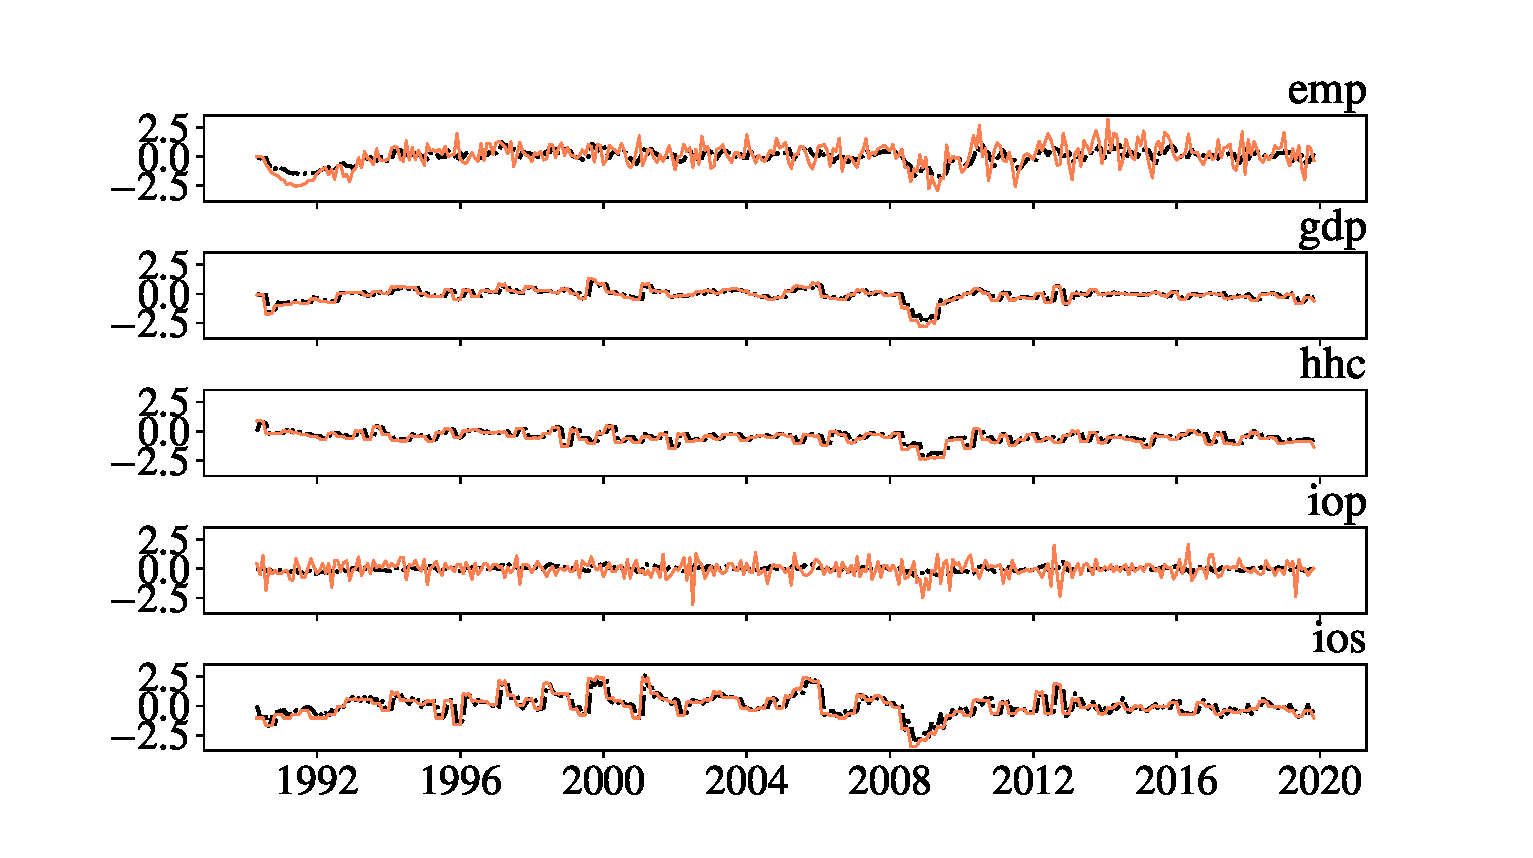
\includegraphics[width=\textwidth]{fcasts.eps} 
	\caption{Example figure. \label{fig:example}}
\end{figure}

\begin{figure}[h]
	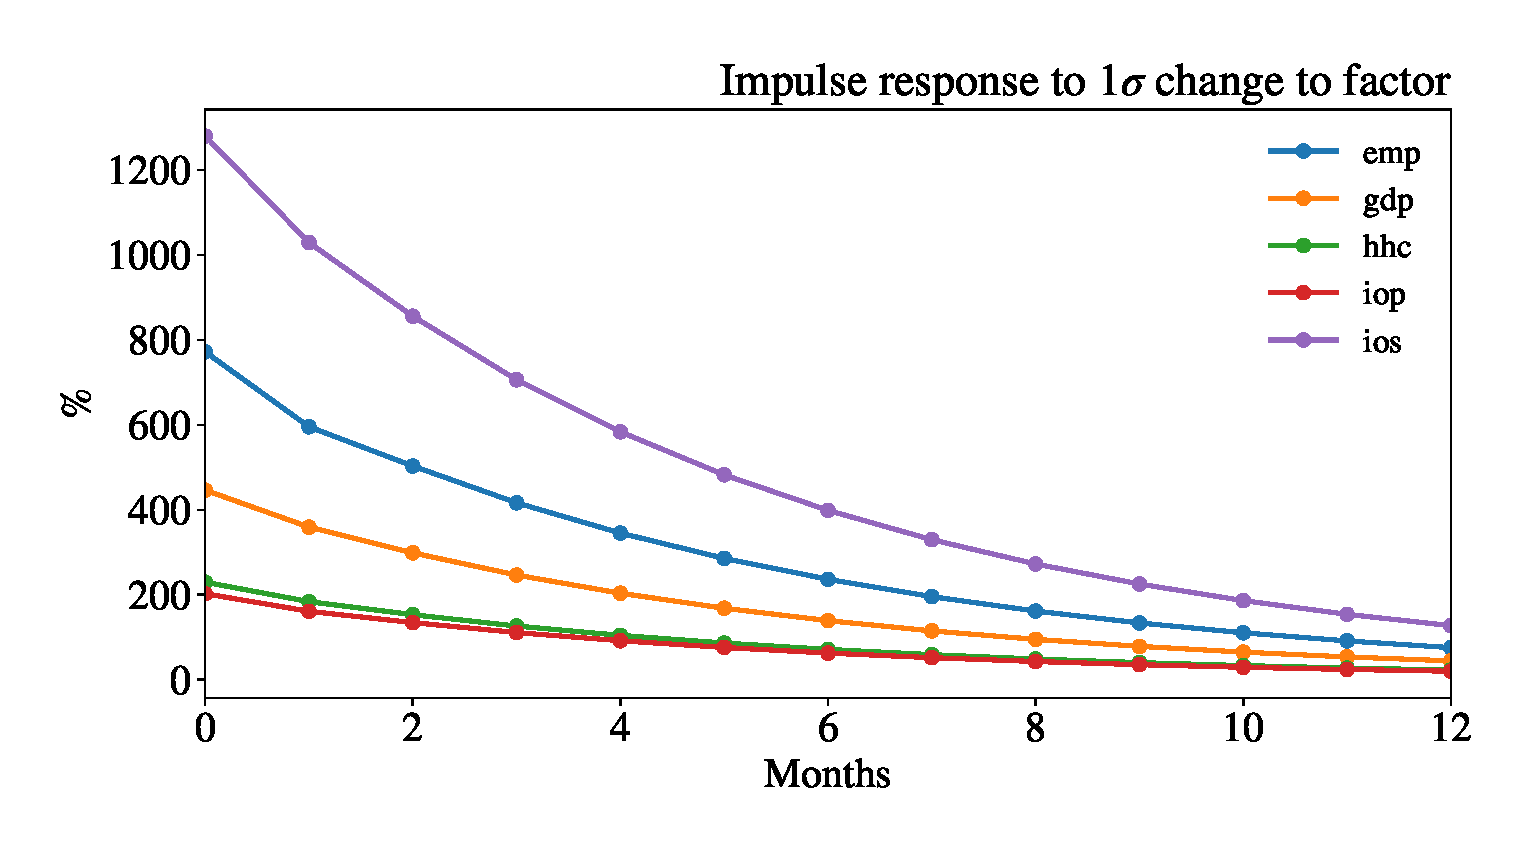
\includegraphics[width=\textwidth]{df_irfs.eps} 
	\caption{Example figure. \label{fig:example}}
\end{figure}

\newpage
\singlespacing 
\bibliographystyle{aea}
%\bibliography{bibliography.bib}

\onehalfspacing

%%%%%%%%%%%%%%%%%%%%%%%%%%%%%%%%%%
%%Figures and tables
%%%%%%%%%%%%%%%%%%%%%%%%%%%%%%%%%%

%\input{Figures.tex}
%\input{Tables.tex}

%%%%%%%%%%%%%%%%%%%%%%%%%%%%%%%%%
%Appendices
%%%%%%%%%%%%%%%%%%%%%%%%%%%%%%%%%

\clearpage  
\appendix

% Appendix number figs and tables within sections
\renewcommand\thefigure{\thesection.\arabic{figure}}
\setcounter{figure}{0}

\renewcommand\thetable{\thesection.\arabic{table}}
\setcounter{table}{0}


\clearpage
\begin{center}
\vspace{-1.8cm}{\LARGE \textbf{PAPER TITLE}}\medskip \\
	\Large \textbf{Online Appendix} \bigskip \\
\large AUTHOR NAME 1 \hspace{0.3cm} AUTHOR NAME 2 \hspace{0.3cm} AUTHOR NAME 3 \hspace{0.3cm} AUTHOR NAME 4 \bigskip
	
\end{center}


%\input{Appendix_text.tex}

%\clearpage
%\input{Appendix_figures.tex}

%\clearpage
%\input{Appendix_tables.tex}




\end{document}
